%%% Local Variables:
%%% mode: latex
%%% TeX-master: "../doc"
%%% coding: utf-8
%%% End:
% !TEX TS-program = pdflatexmk
% !TEX encoding = UTF-8 Unicode
% !TEX root = ../doc.tex

Im folgenden Abschnitt werden die verschiedenen Grundlagen für die Entwicklung eines LOD Systems kurz erläutert. Die Themen sind soweit als möglich voneinander getrennt.

\section{3D-Modelle}
Ein Modell stellt ein Objekt aus der realen Welt vereinfacht dar.
3D-Modelle können vereinfacht als Gruppe von Punkten definiert werden.
Um im dreidimensionalen Raum Objekte visualisieren zu können sind mindestens drei Punkte notwendig.
Punkte von 3D-Modellen werden im folgenden als Vertex (Eckpunkte) bezeichnet und können als Vektor definiert werden.
So können wir einen Vertex am Ursprung eines Koordinatensystems definieren als:
$$ V =
\begin{bmatrix}
  0 \\
  0 \\
  0
\end{bmatrix}
$$
Eine Sammlung von drei \e{Vertices} bildet ein \e{Triangle} (Dreieck). Hiermit kann ein \e{Triangle} generell wie folgt definiert werden:
$$ T =
\begin{bmatrix}
  V \\
  V \\
  V
\end{bmatrix}
$$
Um komplexere Formen wie Vierecke (\e{Quads}) zu bilden, werden jeweils mehrere \e{Triangle} kombiniert. Abbildung \ref{fig:modelSimpleTriangulation} zeigt die Vereinfachung eines \e{Quads} in zwei \e{Triangle}.
\begin{figure}[H]
  \centering
  \begin{subfigure}{.5\textwidth}
    \centering
    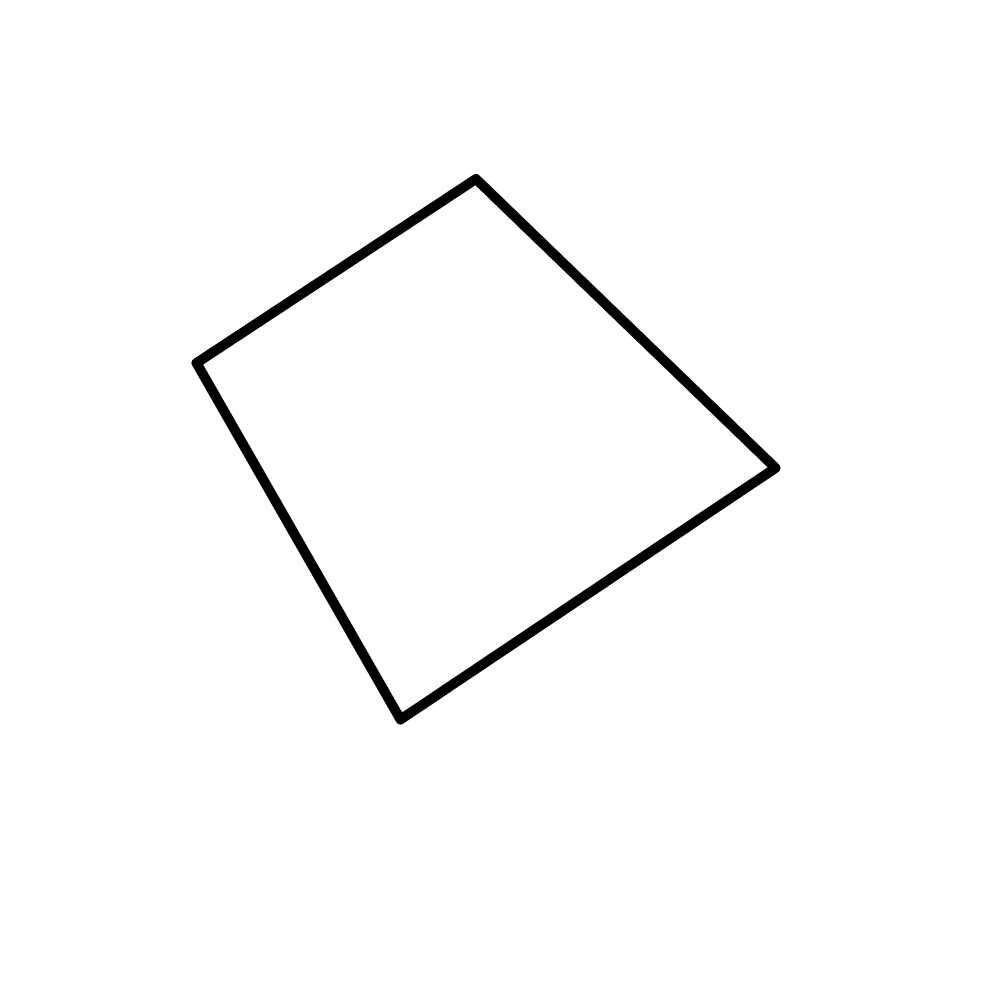
\includegraphics[width=.8\linewidth]{grundlagen/model/polygon.png}
    \caption{Polygon}
  \end{subfigure}%
  \begin{subfigure}{.5\textwidth}
    \centering
    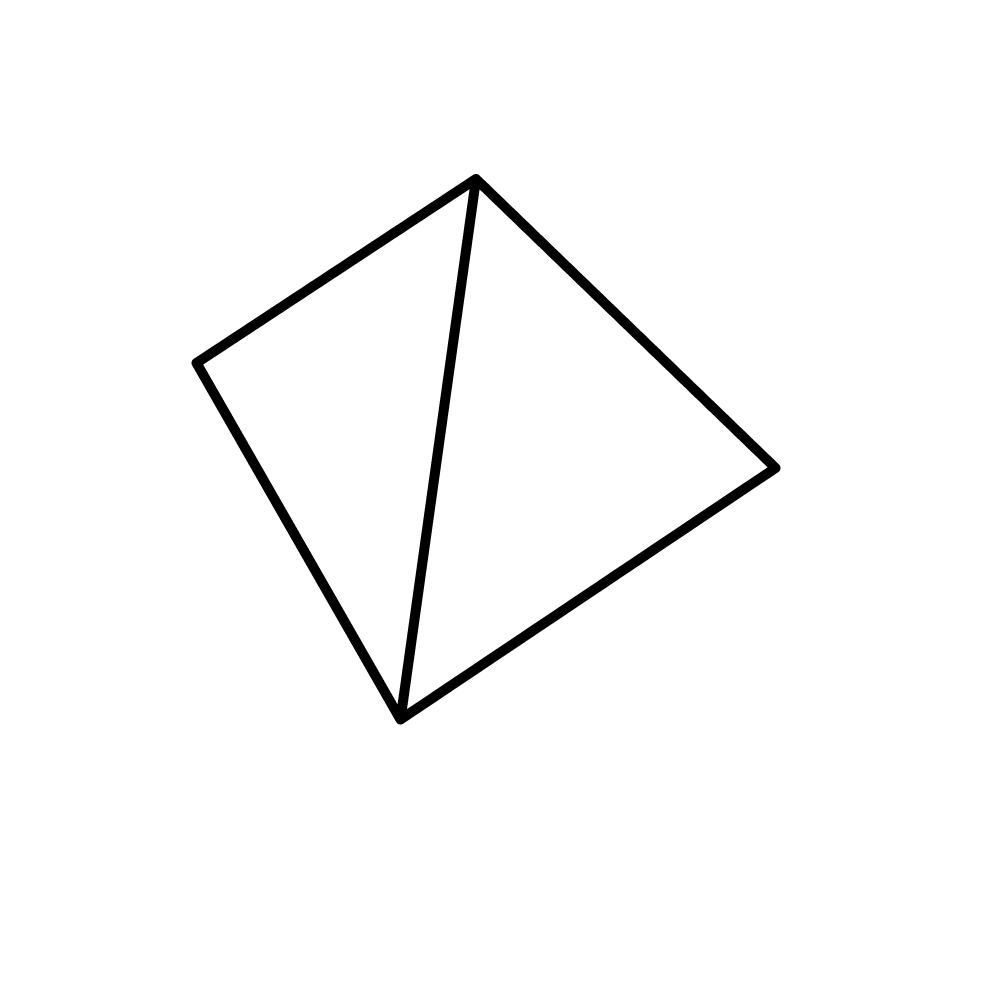
\includegraphics[width=.8\linewidth]{grundlagen/model/polygon-triangulation.png}
    \caption{Polygon als Sammlung von Triangles}
  \end{subfigure}
  \caption{Vereinfachung von Polygone als Sammlung von \e{Triangles}}
  \label{fig:modelSimpleTriangulation}
\end{figure}

Für eine Sammlung von Punkten wird generell der Term Polygon verwendet.
Ein Modell besteht aus einer beliebigen Anzahl Polygone.

Die Verbindung zwischen zwei Vertices ist eine sogenannte Edge (Kante).
Verbindet man die Punkte eines Polygons und füllt die Fläche, ergibt sich schlussendlich ein Face (Fläche).

\paragraph{Weitere Attribute}
Neben den geometrischen Attributen verfügt ein Modell ebenfalls über visuelle Attribute.

So wird für jeden Vertex ein sogenannter \e{Normal} definiert. Ein \e{Normal} ist ein Vektor der im einfachsten Fall senkrecht zu den zwei an diesem Vertex verbundenen Edges verläuft. In der Geometrie ist dies auch bekannt als Normale. \e{Normals} werden häufig für das Berechnen von Reflexionen verwendet.
\e{Normals} werden auch für gewisse Performanz Optimierungen eingesetzt, dazu mehr in \autoref{chap:backfaceCulling}.

Um die Oberfläche von Modellen zu definieren wird häufig ein sogenanntes \fgls{Texture Mapping}{Verfahren, mittels 2D-Bildern 3D-Objekte zu gestalten} durchgeführt. Hierfür sind zusätzliche Informationen für ein Modell notwendig. In der Praxis finden viele weitere Methoden Anwendung, auf diese wird jedoch hier nicht weiter eingegangen.

\paragraph{Abgrenzung}
Diese Sektion erläuterte die für diese Arbeit relevanten polygonale Modelle. Alternativen wie zum Beispiel \e{Point Clouds}, welche das Resultat von 3D-Scans sind, werden nicht weiter erläutert. Auch andere Methoden wie \e{NURBS}, welche Modelle mithilfe von mathematisch definierten Flächen modelliert, werden aussen vor gelassen.

\paragraph{Formate}
Um ein 3D Modell in einer Anwendung zu verwenden, muss ein entsprechendes Format verwendet werden. Hierfür steht eine Vielzahl von Optionen zur Auswahl. Aufgrund der Menge wird hier jedoch nur oberflächlich auf die bekanntesten Formate eingegangen.

\subparagraph{OBJ}
Wavefront OBJ ist ein offenes Dateiformat das von Wavefront Technologies 1989 entwickelt wurde. Das Format ist jedoch speichertechnisch ineffizient und verfügt zudem nur über ein limitiertes Feature Set. Des Weiteren gibt es keine zentrale Instanz, welche eine Spezifikation liefert und Informationen sind deshalb schwerer zu finden. \cite{objSpec}

\subparagraph{FBX}
FBX ist ein proprietäres Format, welches von Autodesk verwaltet wird. Das Verwenden von FBX Daten ist jedoch offiziell nur mit einer C++ FBX SDK möglich, welche für das Web nicht geeignet ist. Aufgrund der proprietären Natur gibt es keine Bestrebungen das Format offener zu gestalten.

\subparagraph{glTF}
Seit 2015 gibt es ein offenes, modernes sowie auf optimale Speichernutzung fokussiertes Format: glTF. Dieses Format wird von der Khronos Gruppe entwickelt. \cite{gltf1Spec} In dieser Arbeit wird es als Austauschformat verwendet, deshalb wird im folgenden genauer auf das Format eingegangen.

Die meisten 3D-Grafikprogramme wie Blender (.blend) verwenden ihre eigenen Dateiformate. Diese Dateiformate sind jedoch für den Einsatz in einer Applikation ungeeignet da sie insbesondere nicht für die Laufzeitperformanz optimiert sind. Deswegen brauchte es für jedes Eingangsformat für jedes Ausgangsformat einen \e{converter}, wie in Abbildung \ref{fig:contentPipelineWithoutGltf} ersichtlich.

\begin{figure}[H]
  \centering
  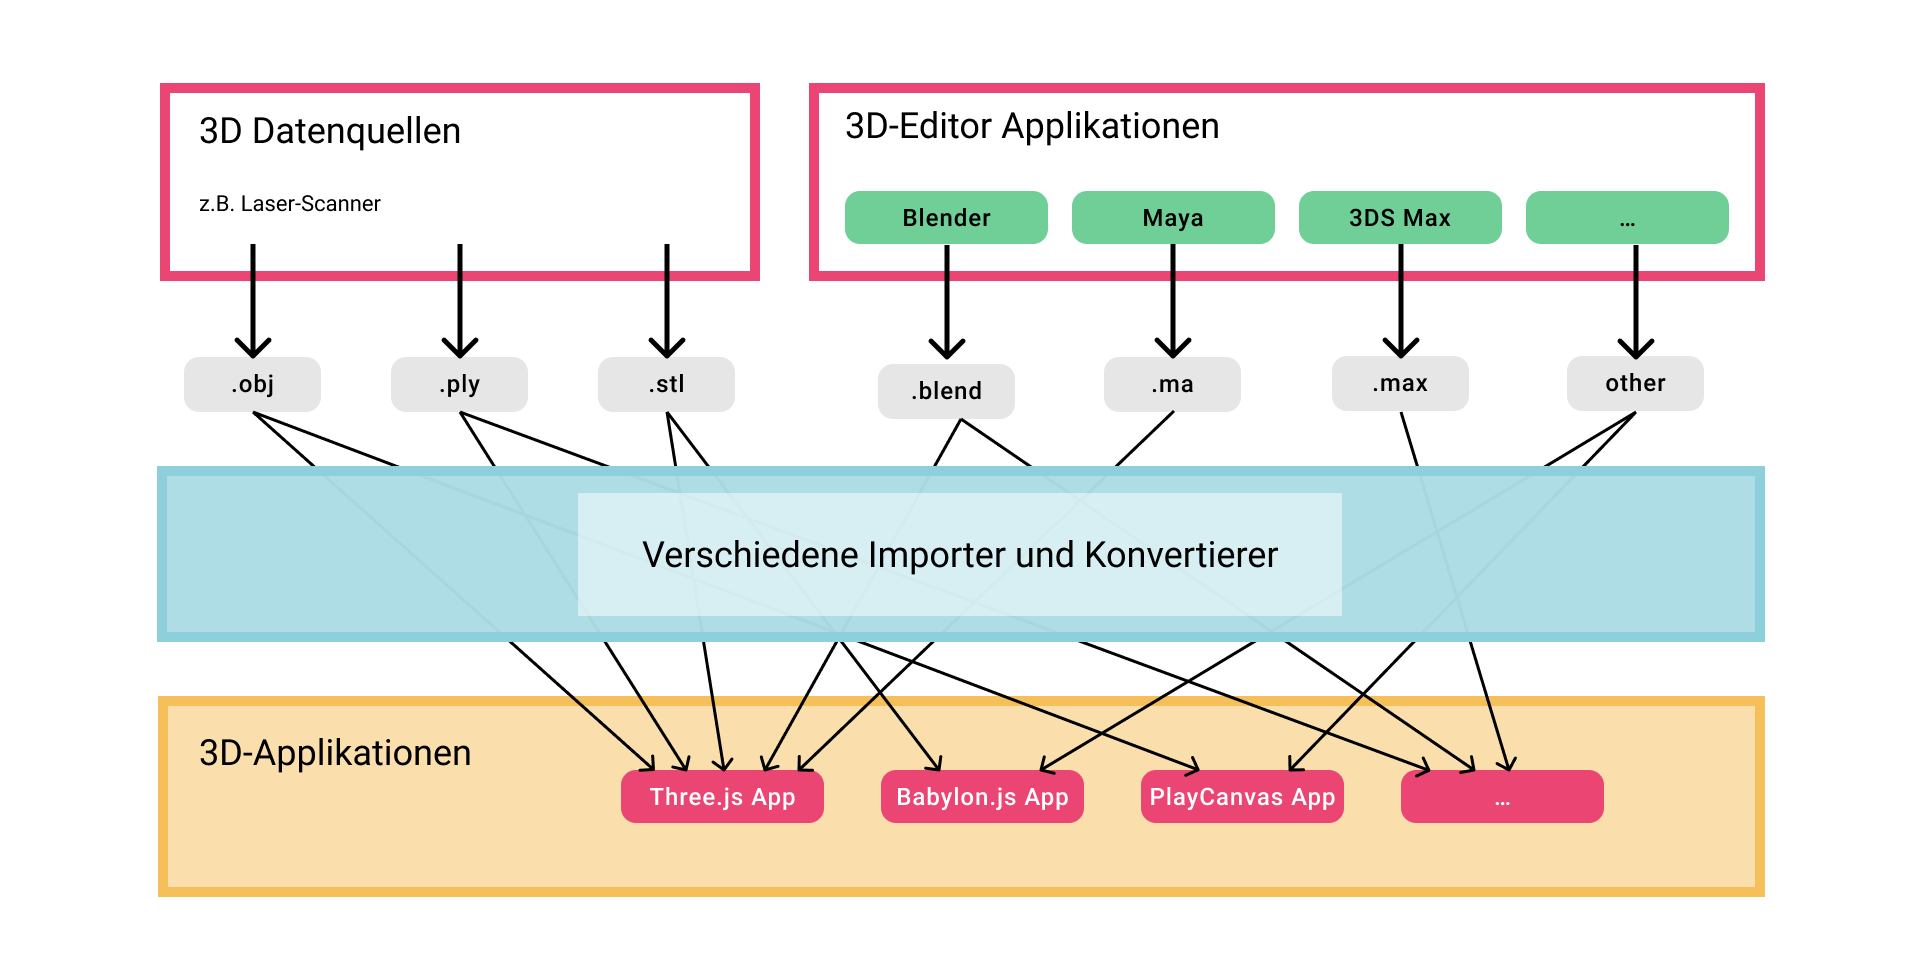
\includegraphics[width=0.8\columnwidth]{grundlagen/gltf/contentPipeline.png}
  \caption{Convertierungspipeline vor glTF \cite{gltf1Spec}}
  \label{fig:contentPipelineWithoutGltf}
\end{figure}

Durch die immer breiter werdende Nachfrage nach 3D-Applikationen wurde ein Format benötigt, dass zum einen Applikationsunabhängig verwendet und zum anderen performant im Web eingesetzt werden kann. \cite{gltf1Spec}
Durch diese Abstraktion kann eine Vielzahl \e{converter} vermieden werden und nur wenige, sehr spezifische Dateiformate benötigen noch einen einzigen \e{converter}. Diese neue Pipeline ist in Abbildung \ref{fig:contentPipelineWithGltf} dargestellt. \cite{gltf1Spec}
\begin{figure}[H]
  \centering
  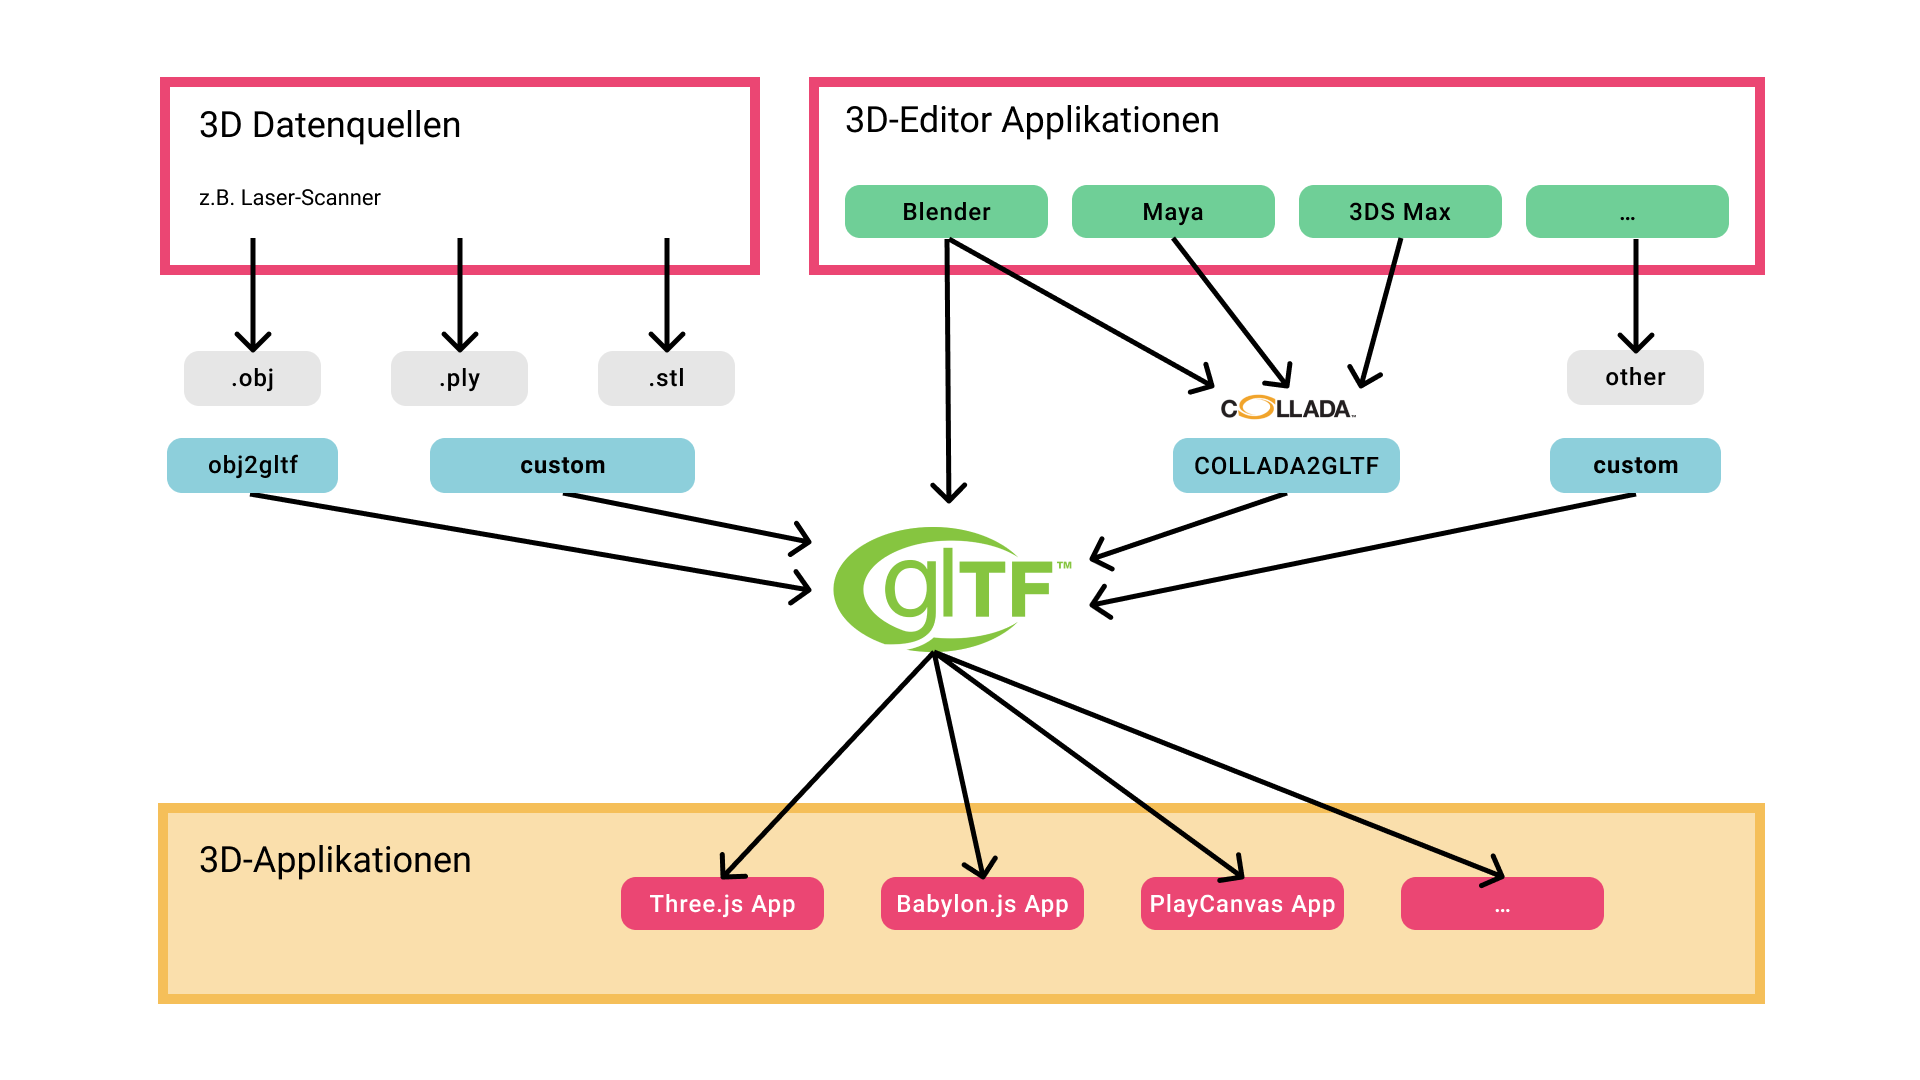
\includegraphics[width=0.8\columnwidth]{grundlagen/gltf/contentPipelineWithGltf.png}
  \caption{Convertierungspipeline mit glTF \cite{gltf1Spec}}
  \label{fig:contentPipelineWithGltf}
\end{figure}

Die Basisstruktur von glTF basiert auf JSON. Darin ist die komplette Szenerie des Modells beschrieben und in Abbildung \ref{fig:gltfDatastructure} aufgezeigt.\cite{gltf1Spec}
\begin{figure}[H]
  \centering
  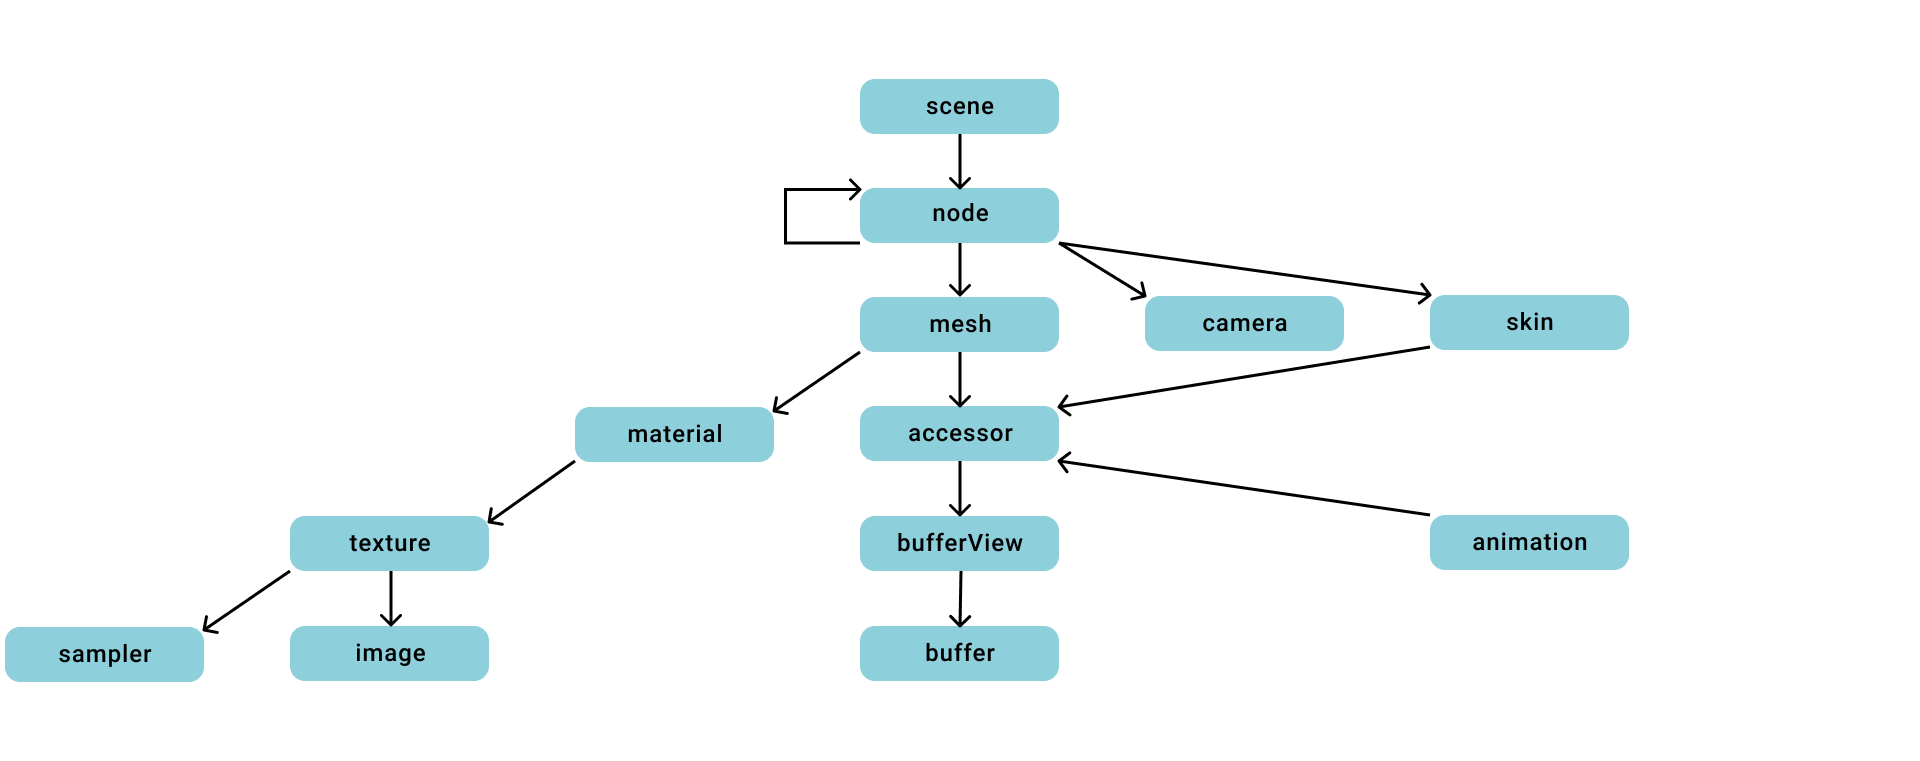
\includegraphics[width=0.8\columnwidth]{grundlagen/gltf/gltfJsonStructure.png}
  \caption{glTF Datenstruktur \cite{gltf1Spec}}
  \label{fig:gltfDatastructure}
\end{figure}

Die wichtigsten Elemente dieser Struktur kurz erläutert:
\begin{itemize}
  \item \textbf{Scene}: Einstiegspunkt der Szenerie und verweist auf alle Top-Level \e{nodes}.
  \item \textbf{Node}: Kann eine Transformation (Rotation, Translation oder Skalierung) beinhalten oder eine Kamera, \e{Skin}, Animation, ein \e{Mesh} oder \e{Childnodes} referenzieren.
  \item  \textbf{Mesh}: Beschreibt ein geometrisches Objekt und verweist auf \e{accessor}, welcher die effektiven geometrischen Daten beinhaltet und auf \e{material}, das beschreibt, wie das Objekt beim Rendern aussehen soll.
  \item \textbf{Accessor}: Verweis auf die Binärdaten (\e{BufferView}), welche die effektiven Eigenschaften für \e{meshes}, \e{skins} und \e{animations} kompakt beinhaltet.
  \item \textbf{BufferView}: Definiert eine Ansicht (Länge, Ort, Typ)auf einen \e{Buffer}.
  \item \textbf{Buffer}: Verweist auf einen Block von Binärdaten, welchen die effektiven Daten des 3D-Modells platzsparend beinhaltet.
  \item \textbf{Material}: Definiert die visuellen Attribute eines \e{Mesh}.
  \item Weitere Elemente, welche im Rahmen dieser Arbeit nicht relevant sind und nicht im Detail betrachtet werden, sind: \e{camera}, \e{skin}, \e{animation}, \e{texture}.
\end{itemize}

\section{Transformation von Modellen}

Um ein Modell vereinfachen zu können, muss es verändert werden.
Diese Veränderungen können in Basis Operationen vereinfacht erläutert werden.

Im Folgenden werden Transformationen mithilfe einer 2D Visualisierung erläutert. Das Modell kann jedoch ebenfalls im dreidimensionalen Raum sein – die Funktionsweise bleibt identisch.

Für die folgenden Beispiele wird jeweils das Modell aus Abbildung \ref{fig:transformationOriginal} verwendet.

\begin{figure}[H]
  \centering
  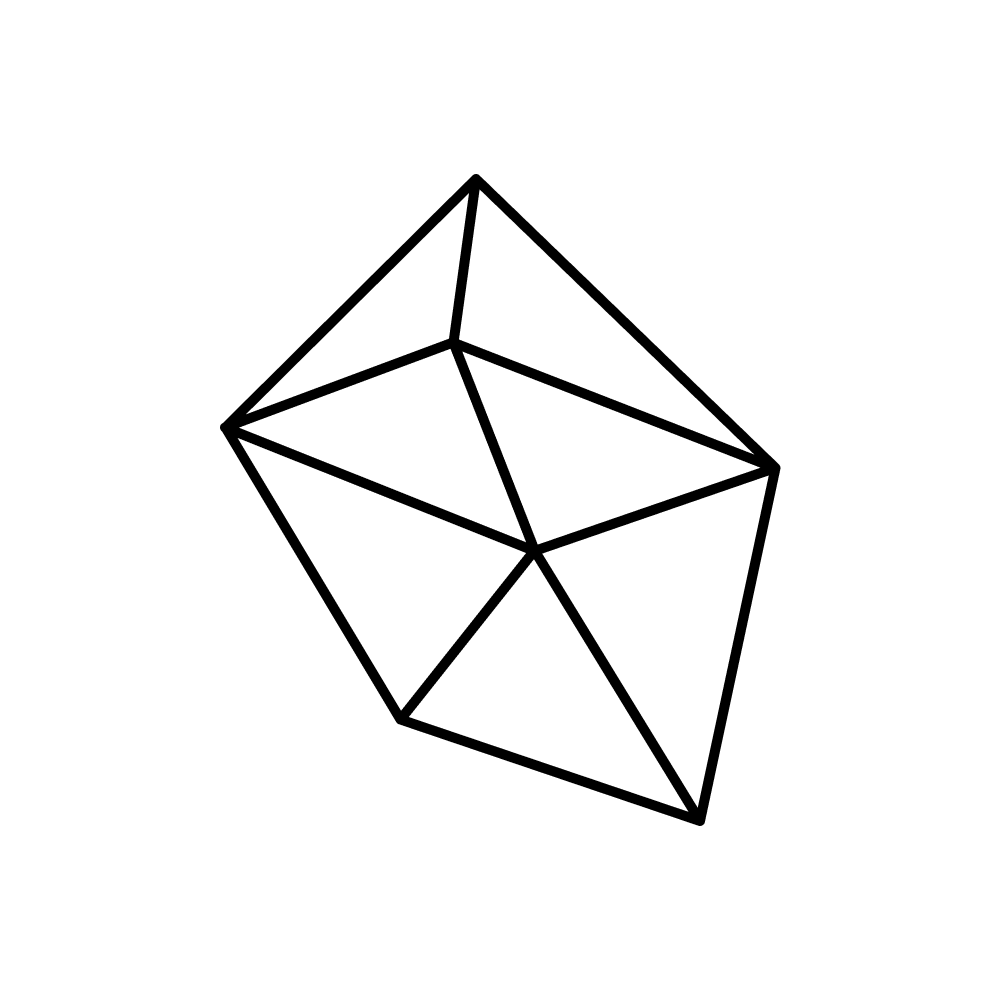
\includegraphics[width=0.4\columnwidth]{grundlagen/transformationen/original.png}
  \caption{Modell Basis}
  \label{fig:transformationOriginal}
\end{figure}

\paragraph{Edge Collapse}
Hierbei werden zwei nebeneinanderliegende \e{Vertices} kombiniert. Durch diese Operation kann ein \e{Vertex} entfernt werden. In Abbildung \ref{fig:transformationEdgeCollapse} kann die Anzahl \e{Triangles} um zwei verringert werden. Beim \e{Edge Collapse} wird ein neuer \e{Vertex} definiert und zwei bestehende entfernt. Die Anzahl entfernter \e{Triangles} ist abhängig von der Situation. Unter Umständen kann so auch nur ein einzelner \e{Triangle} entfernt werden.
Die Umkehrfunktion nennt man Vertex Split.

\begin{figure}[H]
  \centering
  \begin{subfigure}{.5\textwidth}
    \centering
    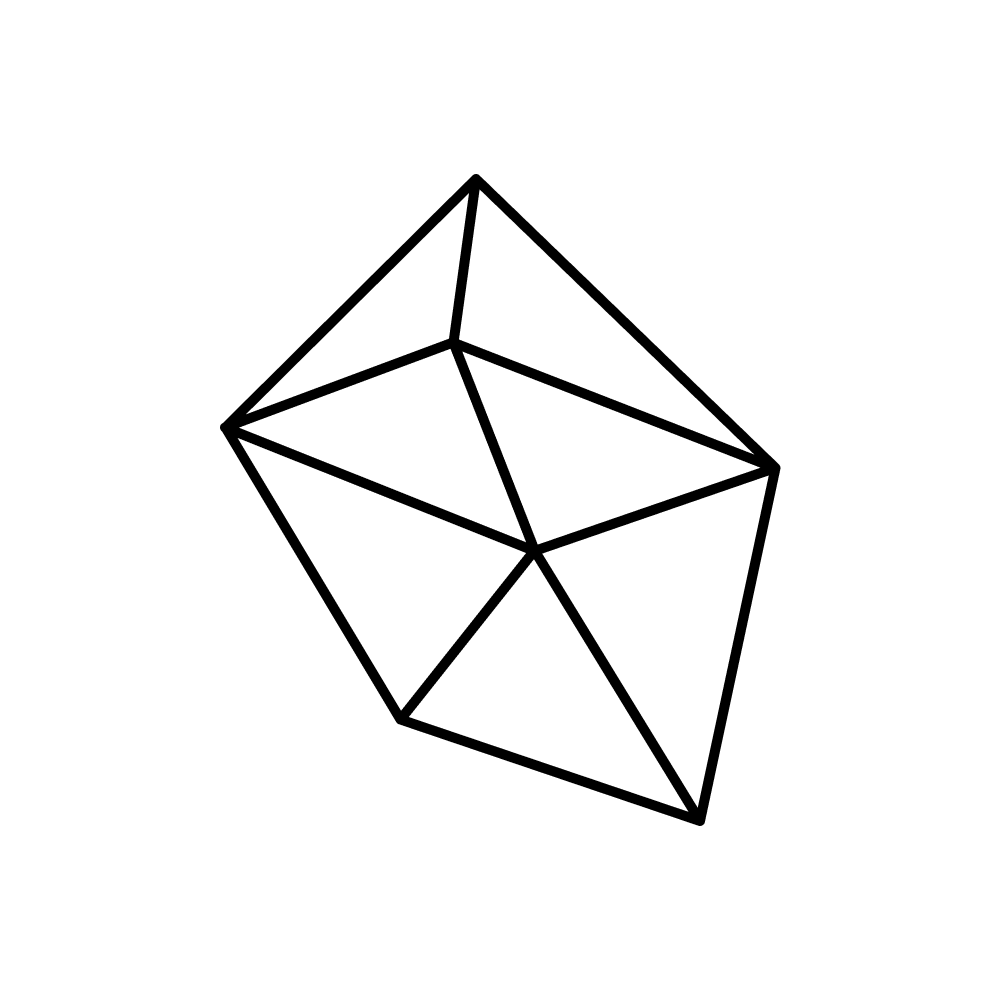
\includegraphics[width=.8\linewidth]{grundlagen/transformationen/original.png}
    \caption{Modell Ausgangslage}
  \end{subfigure}%
  \begin{subfigure}{.5\textwidth}
    \centering
    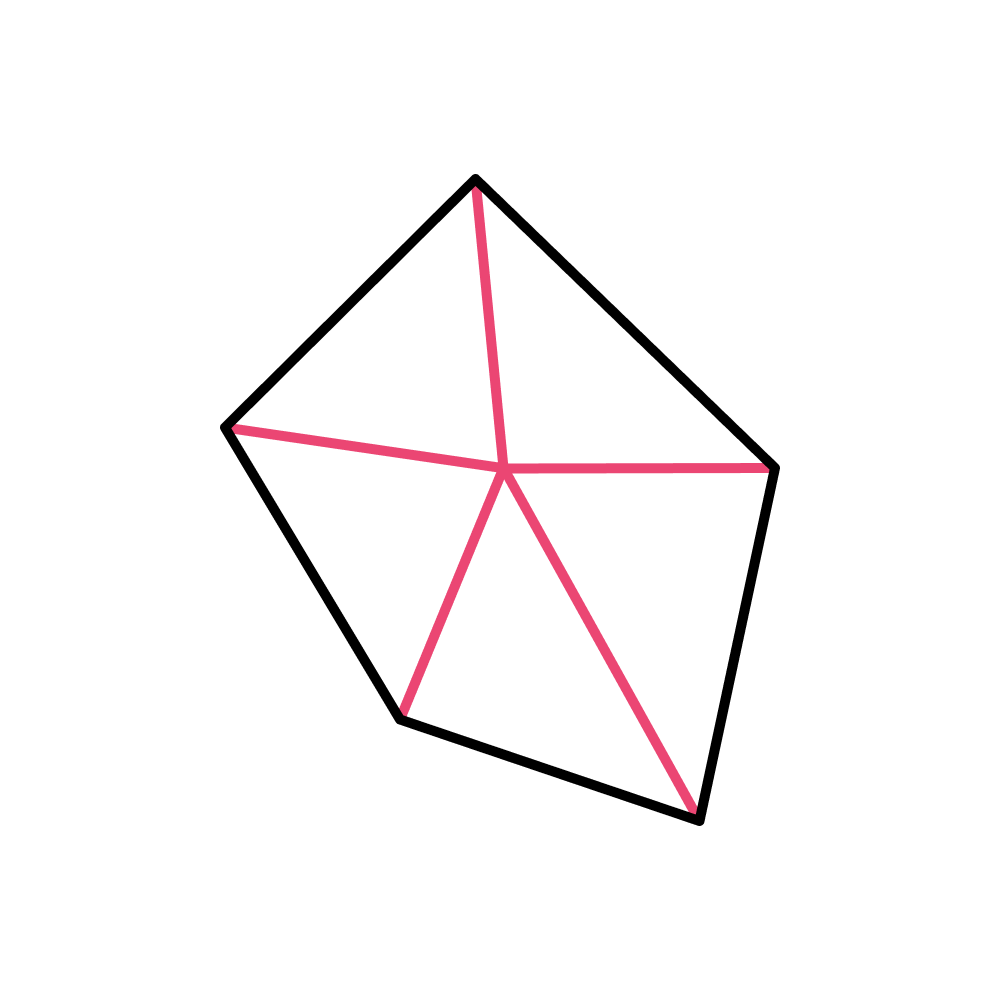
\includegraphics[width=.8\linewidth]{grundlagen/transformationen/edge-collapse.png}
    \caption{Edge Collapse}
  \end{subfigure}
  \caption{Transformation mittels Edge Collapse}
  \label{fig:transformationEdgeCollapse}
\end{figure}

\paragraph{Halfedge Collapse}
Hierbei wird ein Vertex direkt entfernt und alle Edges auf einen danebenliegenden Vertex zusammengelegt. Bei dieser Operation muss kein neuer \e{Vertex} definiert werden, sondern ein bereits bestehender \e{Vertex} kann wiederverwendet werden. Wie in Abbildung \ref{fig:transformationHalfedgeCollapse} ersichtlich, können auch in diesem Fall zwei \e{Triangles} entfernt werden.

\begin{figure}[H]
  \centering
  \begin{subfigure}{.5\textwidth}
    \centering
    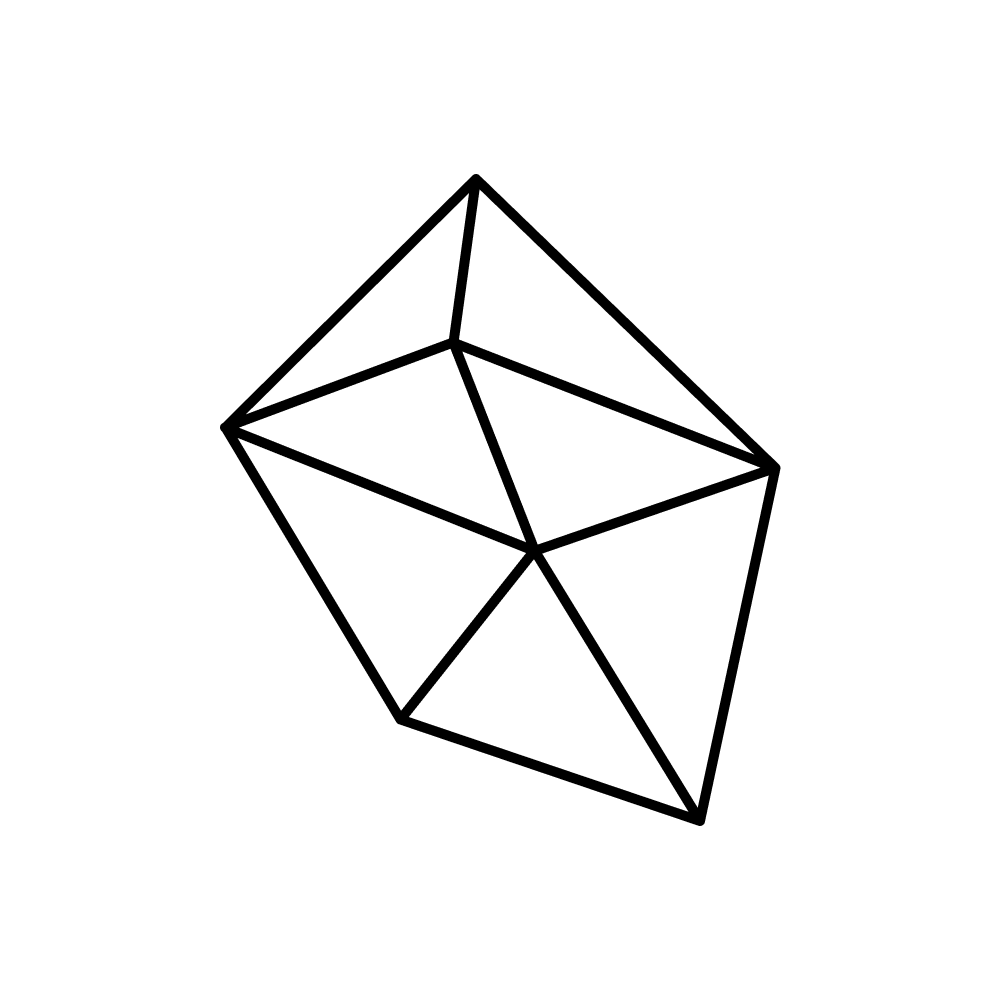
\includegraphics[width=.8\linewidth]{grundlagen/transformationen/original.png}
    \caption{Modell Ausgangslage}
  \end{subfigure}%
  \begin{subfigure}{.5\textwidth}
    \centering
    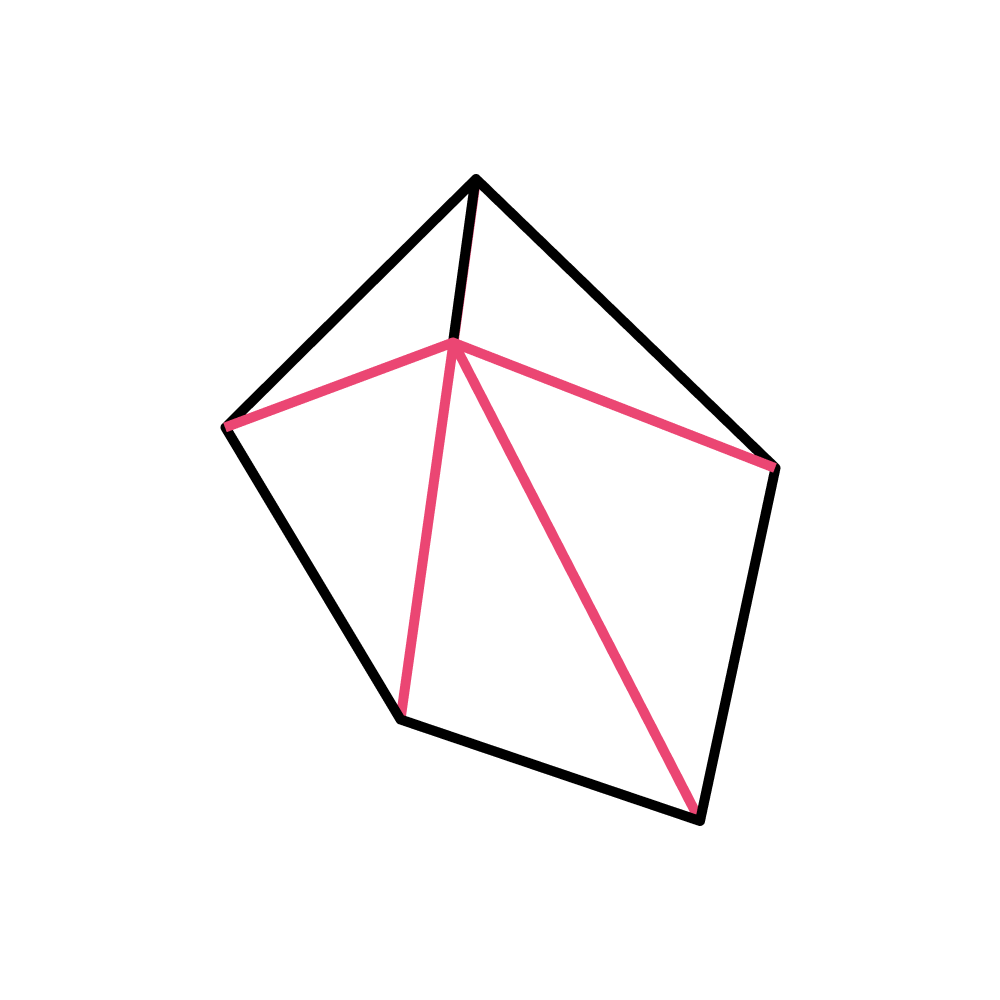
\includegraphics[width=.8\linewidth]{grundlagen/transformationen/half-edge-collapse.png}
    \caption{Halfedge Collapse}
  \end{subfigure}
  \caption{Transformation mittels Halfegde Collapse}
  \label{fig:transformationHalfedgeCollapse}
\end{figure}

\paragraph{Vertex Removal}
Hierbei wird ein Vertex entfernt und das Resultat neu trianguliert. Triangulation ist ein Verfahren, um ein Polygon in \e{Triangles} aufzuteilen.
In Abbildung \ref{fig:transformationVertexRemovalOriginal} wird der zentrale Vertex entfernt. Anschliessend werden alle \e{Triangles} an diesem Punkt entfernt. Das dabei entstehende Loch wird neu mit \e{Triangles} gefüllt. Der neu triangulierte Polygon ist in Abbildung \ref{fig:transformationVertexRemovalFinal} ersichtlich.

\begin{figure}[H]
  \centering
  \begin{subfigure}{.5\textwidth}
    \centering
    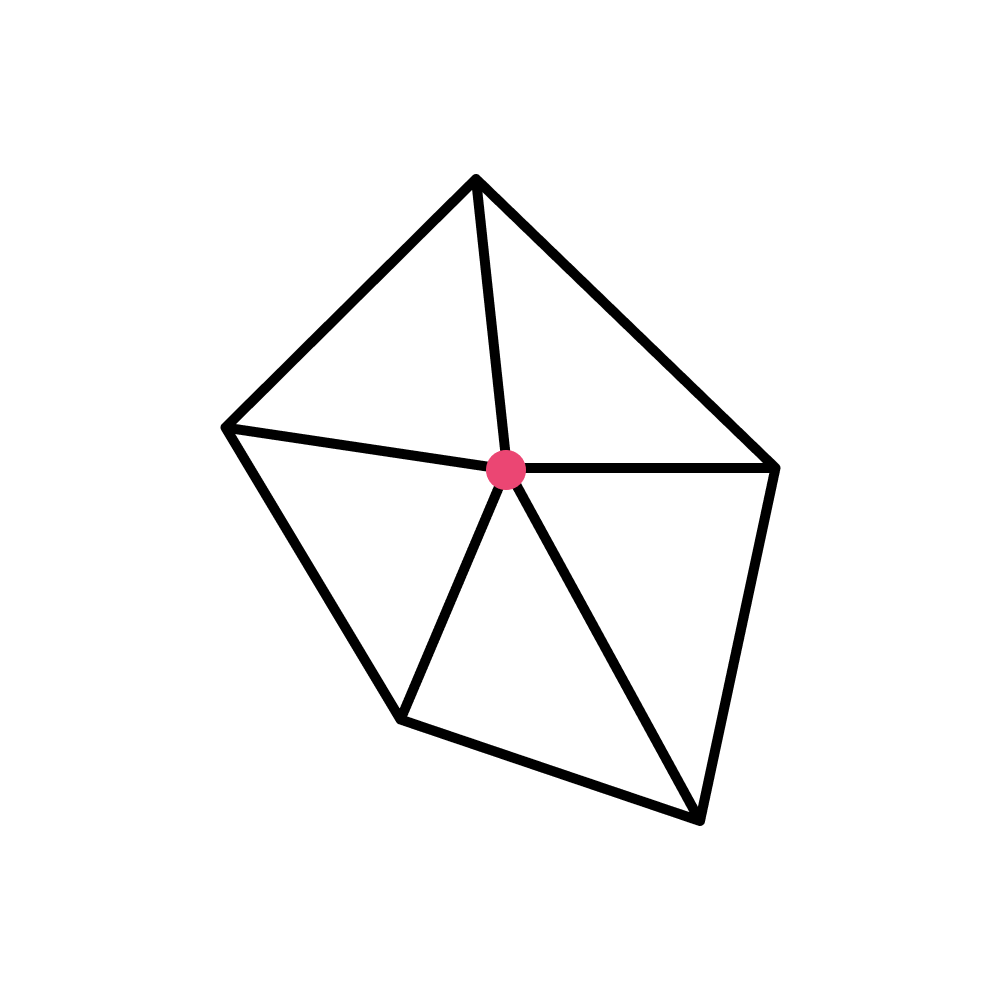
\includegraphics[width=.8\linewidth]{grundlagen/transformationen/vertex-removal-original.png}
    \caption{Modell Ausgangslage}
    \label{fig:transformationVertexRemovalOriginal}
  \end{subfigure}%
  \begin{subfigure}{.5\textwidth}
    \centering
    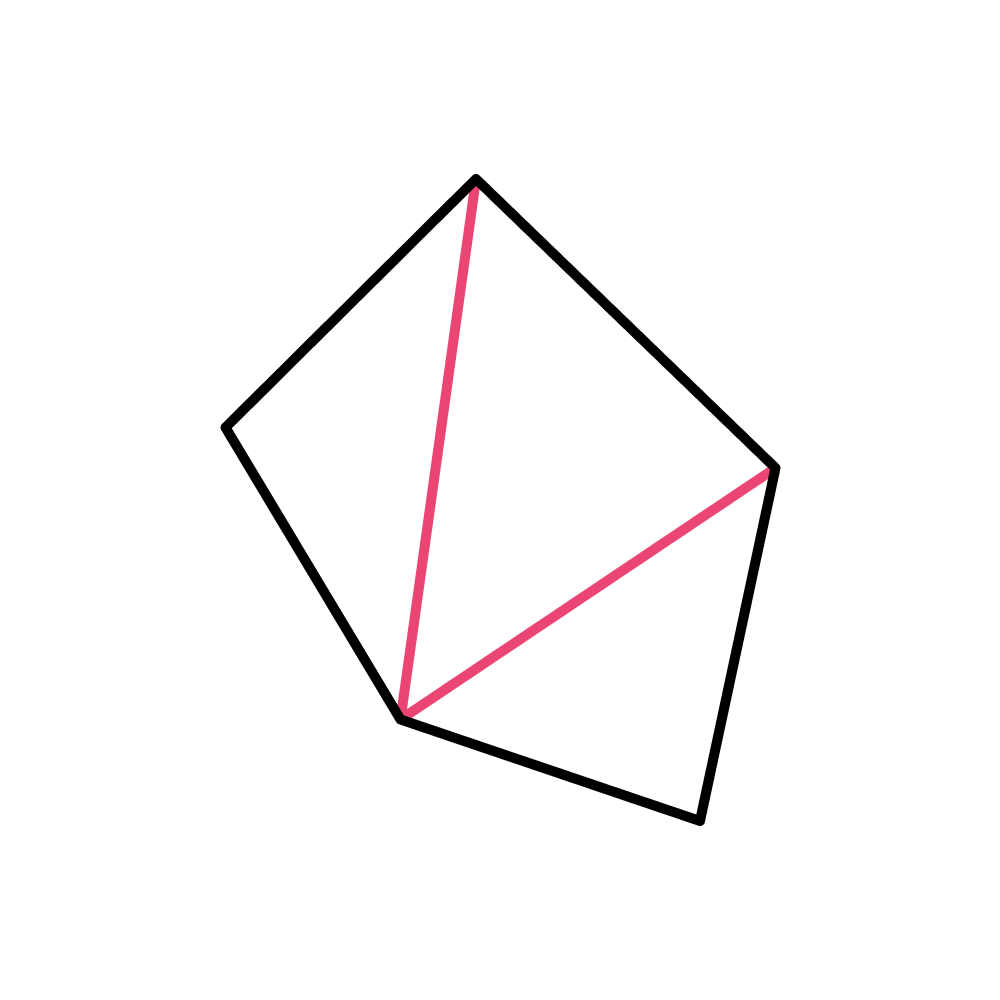
\includegraphics[width=.8\linewidth]{grundlagen/transformationen/vertex-removal-final.png}
    \caption{Vertex Removal}
    \label{fig:transformationVertexRemovalFinal}
  \end{subfigure}
  \caption{Transformation mittels Vertex Removal}
  \label{fig:transformationVertexRemoval}
\end{figure}

\section{Grafikpipeline}
Die Grafikpipeline ist zuständig um eine definierte Szene auf einem Ausgabegerät zu visualisieren. Die verschiedenen Schritte werden im folgenden Abschnitt kurz erläutert. Es wird dabei ein simples 3D-Modell auf einem 2D-Display, wie zum Beispiel einem Monitor, visualisiert. Die verschiedenen Schritte sind in Abbildung \ref{fig:renderingPipelineOverview} aufgezeigt.

\begin{figure}[H]
  \centering
  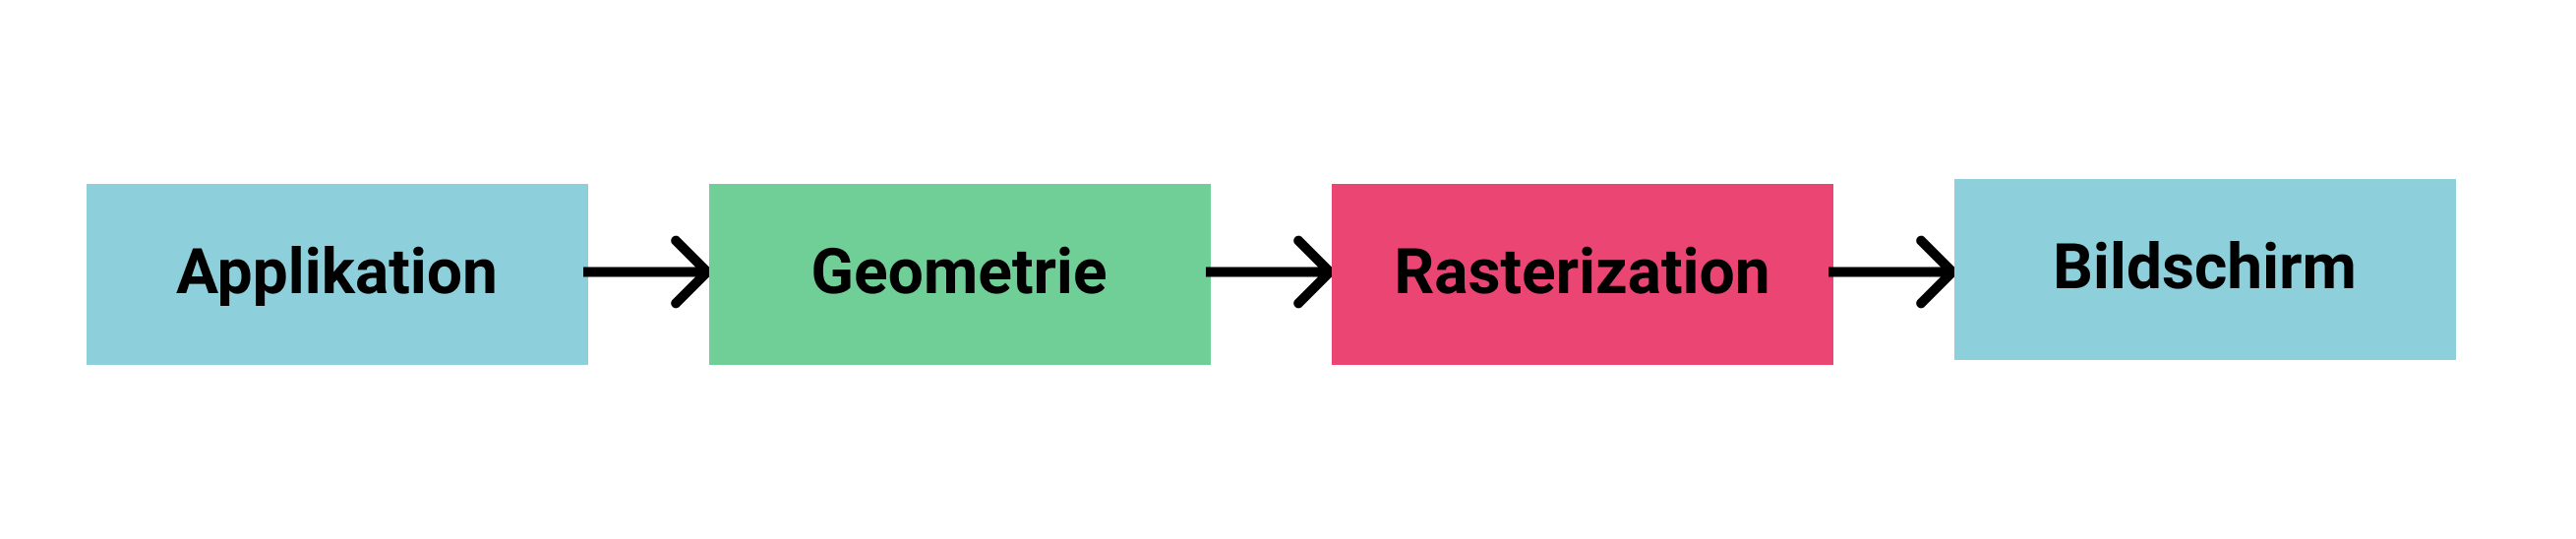
\includegraphics[width=0.8\columnwidth]{grundlagen/pipeline/graphics-pipeline.png}
  \caption{Schritte einer Realtime Rendering Pipeline}
  \label{fig:renderingPipelineOverview}
\end{figure}

\paragraph{Applikation}
Im ersten Schritt wird die Szenerie aufbereitet, Modelle in den Arbeitsspeicher geladen, Positionen und Rotationen der Modelle definiert. Diese Schritte werden auf der CPU durchgeführt. Ein Beispiel für das aufsetzen eines einfachen \e{Triangles} bestehnd aus drei \e{Vertices} ist in Abbildung \ref{fig:geometryDefinition} ersichtlich.

\begin{figure}[H]
\begin{lstlisting}
const vertices = new Float32Array([
  -1, 1, 0, // vertex 0
  -1, -1, 0, // vertex 1
  1, -1, 0 // vertex 2
]);

const indices = new Uint16Array(
  [0, 1, 2] // triangle 0
);
\end{lstlisting}
\caption{Definition eines Triangles}
\label{fig:geometryDefinition}
\end{figure}

\paragraph{Vertexshader}
Anschliessend werden die Daten an die GPU gesendet. Der erste Schritt ist der sogenannte Vertexshader. Auftrag des Vertexshaders ist es, die \e{Vertices} zu transformieren. Die Modelle werden ausgerichtet, die Beleuchtung bestimmt und die 2D-Projektion vorgenommen. Ein Beispiel für einen simplen Vertexhsader ist in Abbildung \ref{fig:vertexShader} ersichtlich.

\begin{figure}[H]
\begin{lstlisting}
attribute vec3 coordinates;

void main(void) {
  gl_Position = vec4(coordinates, 1.0);
}
\end{lstlisting}
\caption{Vertexshader für die Definition eines Punktes}
\label{fig:vertexShader}
\end{figure}

\paragraph{Fragmentshader}
Durch die Rasterisierung werden kontinuierliche Objekte zu diskreten Fragmenten verarbeitet. Der Fragmentshader generiert die Farbdefinitionen für die einzelnen Pixel. Ein einfaches Beispiel ist in Abbildung \ref{fig:fragmentShader} ersichtlich.

\begin{figure}[H]
\begin{lstlisting}
void main(void) {
  gl_FragColor = vec4(0.0, 0.0, 0.0, 1.0);
}
\end{lstlisting}
\caption{Fragmentshader für das definieren von Farbwerten}
\label{fig:fragmentShader}
\end{figure}


\paragraph{Bildschirm}
Am Schluss wird das vom Fragmentshader generierte Bild auf dem Bildschirm dargestellt.

\section{Performanzoptimierung}
Visualisierungen können zu komplex werden, um jederzeit performant und interaktiv gerendert zu werden.
Insbesondere wenn viele Objekte gleichzeitig sichtbar sind, lohnt es sich Performanzoptimierungen durchzuführen.
Im Idealfall geschieht dies jedoch, ohne dass der Anwender dies bemerkt.

In diesem Abschnitt werden mögliche Ansätze erklärt, welche helfen sollen, die Render-Performanz zu erhöhen. Diese Arbeit konzentriert sich jedoch auf den Ansatz von Level of Detail; die anderen Ansätze werden nur kurz erläutert. Detailliert auf Level of Detail wird in \autoref{chap:lodIntroduction} eingegangen.

\paragraph{Frustum culling}
Polygone, welche nicht im Kamera Frustum enthalten sind, werden bei dieser Methode nicht weiter prozessiert.
Dies reduziert die Anzahl Polygone drastisch.

\begin{figure}[H]
  \centering
  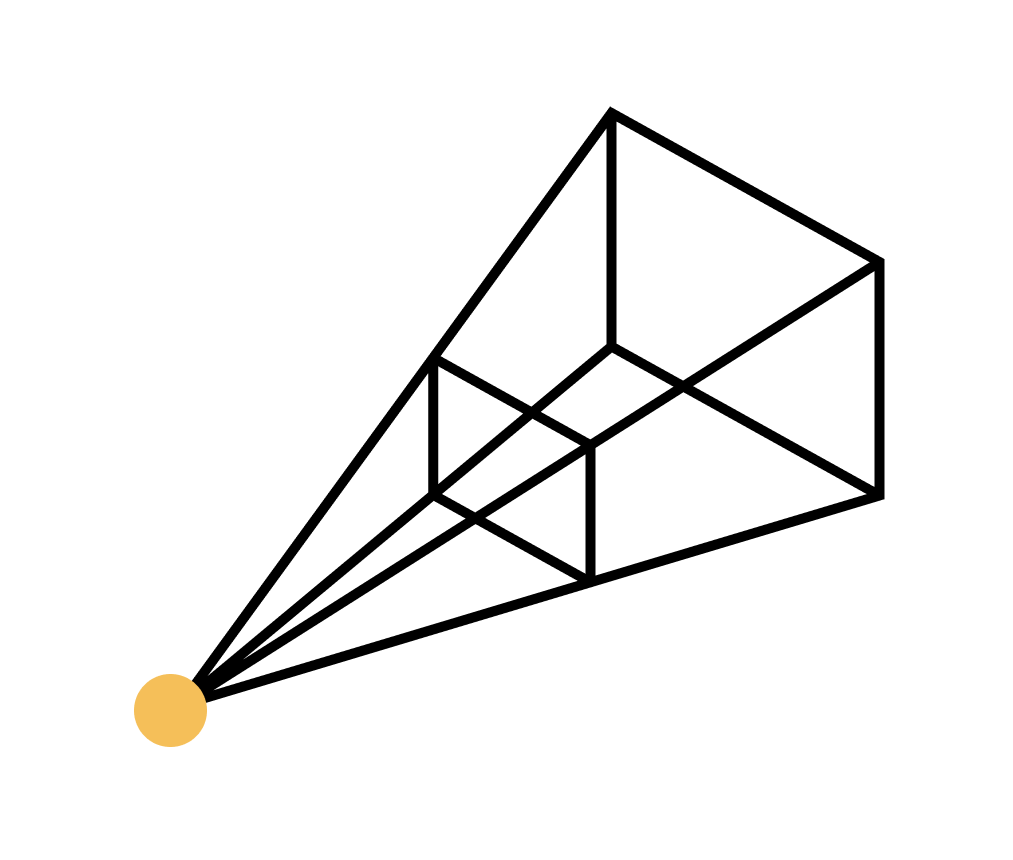
\includegraphics[width=0.5\columnwidth]{grundlagen/Camera-Frustum.png}
  \caption{Kamera Frustum}
  \label{fig:CameraFrustum}
\end{figure}

Ein Frustum ist eine geometrische Form, die einer Pyramide ähnelt, welcher die Spitze abgeschnitten wurde.
Das Kamera-Frustum bezeichnet den Raum, welcher von der Kamera aufgezeichnet wird. Dieser Breich startet eine gewisse Distanz von der Kamera entfernt und endet weit hinten wieder, da nicht bis ins unendliche Objekte sichtbar sind.
Wie in Abbildung \ref{fig:CameraFrustum} zusehen ist, beginnt das Kamera-Frustum in der Nähe der Kamera und dehnt sich ein wenig aus bis es gegen Ende des Spektrums beschränkt wird.

\paragraph{Occlusion culling}
Polygone bzw. Objekte, welche komplett von anderen Objekten überdeckt werden, werden bei dieser Variante nicht prozessiert.

\paragraph{Backface culling}
\label{chap:backfaceCulling}
Bei dieser Methode wird berechnet welche Polygone zur Kamera orientiert sind.
Alle Polygone, welche in die andere Richtung zeigen werden nicht gezeichnet.
Dies ist nicht immer gewünscht, für die meisten Anwendungen ist diese Optimierung jedoch aktiviert.
Als Grundlage für die Berechnung werden die \e{Normals} der \e{Vertices} berücksichtigt.

\paragraph{Parallel rendering}
Auch bekannt unter Distributed Rendering ist der Einsatz von Techniken aus dem Parallel Programming in Visualisierungsanwendungen.

\paragraph{Image-based rendering}
In gewissen Fällen kann das Modellieren übersprungen werden. So kann anhand von Bildmaterial eine 3D-Illusion erzeugt werden.

\section{Einführung Level of Detail}
\label{chap:lodIntroduction}
Als Level Of Detail (LOD) werden die verschiedenen Detailstufen bei der virtuellen Darstellung bezeichnet.
Dies wird verwendet, um die Geschwindigkeit von Anwendungen zu steigern, indem Objekte im Nahbereich detailiert angezeigt werden; wohingegen Elemente im Fernbereich deutlich vereinfacht dargestellt werden.

Ein LOD Algorithmus hat das Ziel für ein gegebenes Modell eine vereinfachte Darstellung zu finden, welche das Original ausreichend annähert. Um diese Approximationen zu generieren, kann eine Vielzahl von Algorithmen verwendet werden. Es gibt verschiedene Ansätze zur Generierung von LODs, welche in \autoref{chap:lodAlgorithmComparison} im Detail erläutert werden.

\begin{figure}[H]
\centering
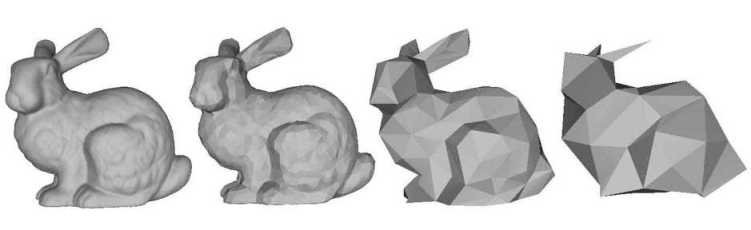
\includegraphics[width=0.8\columnwidth]{LODs-of-a-bunny-model-Courtesy-Stanford-3D-Scanning-Repository-From-left-to-right}
\caption{Level Of Detail Visualisierung vier Hasen}
\label{fig:LevelOfDetailVisualisierungvierHasen}
\end{figure}

Wie in der Abbildung \ref{fig:LevelOfDetailVisualisierungvierHasen} zu erkennen ist, wird von links nach rechts der Detailgrad und somit die Komplexität des Objektes reduziert. Sind es im Bild ganz links noch 69'451 Polygone, wird es bereits im ersten Schritt auf 2'502 Polygone reduziert. Dies ist eine enorme Reduktion von ca. 96.5\%. Im dritten Schritt wird die Anzahl Polygone wiederum um ca. 90\% auf 251 reduziert. Schlussendlich hat das letzte Objekt noch 76 Polygone was knapp 0.1\% der ursprünglichen Anzahl entspricht.

\subsection{Ansätze für LOD Artefakte}
\label{chap:differentLodApproaches}
Es gibt verschiedene Ansätze, 3D-Modelle mittels LOD zu vereinfachen. In diesem Abschnitt werden einige davon detaillierter erläutert so wie ihre Vor- und Nachteile aufgezeigt.

\paragraph{Diskrete LOD (DLOD)}
Bei diskreten LOD werden für ein detailliertes Modell mehrere weniger detaillierte Modelle erstellt.
Abhängig von der Distanz zum Betrachter wird das optimale Modell gewählt. Es sind hierfür nur minimale Anpassungen am \fgls{Scene Graph}{Objektorientierte Datenstruktur zur Beschreibung von 2D- oder 3D-Szenarien} notwendig da ausschliesslich ganze Modelle ausgetauscht werden.
Ein Nachteil sind jedoch merkbare harte Grenzen. Der Benutzer stellt beim umhergehen in der Szene fest, wenn das Modell mit einer einfacheren Version ausgetauscht wird.
Es ist zudem häufig nicht möglich grosse Modelle sinnvoll zu vereinfachen. So ist der Ansatz für Terrain ungeeignet. Ähnlicherweise ist es auch nicht möglich viele sehr kleine Modelle zu kombinieren da jedes Modell unabhängig ist.

\paragraph{Kontinuierliche LOD (CLOD)}
Im Gegensatz zu DLOD wird bei CLOD vereinfachende Veränderungen an einem Modell gespeichert.

Der Hauptunterschied zu DLOD besteht in den weichen Grenzen, so ist es signifikant weniger auffällig da zwischen den verschiedenen Auflösungen interpoliert werden kann.
Der Hauptnachteil ist jedoch, dass diese Interpolation insbesondere Auswirkungen auf die Laufzeit Performanz der Applikation hat.
Das Problem des Clusterings ist auch für diese Variante nicht gelöst.

\paragraph{Hierarchische LOD (HLOD)}
Bei HLOD werden mehrere Objekte in einen Cluster gruppiert.
Diese Methode erlaubt es somit zum Beispiel Terrains optimal abzubilden. So werden Ausschnitte, welche nahe beim Benutzer sind mit hoher Auflösung dargestellt während weiter entferntere Teile der Umgebung mit weniger Details ausgestattet sind.
Zudem ist es möglich viele kleinere Objekte bei entsprechenden Distanzen zu kombinieren.
Der Hauptnachteil liegt darin, dass hierfür signifikante Anpassungen am Scene Graph notwendig sind und für den Entwickler ein spürbarer Unterschied entstehen kann.

\subsection{Vergleich Algorithmen}
\label{chap:lodAlgorithmComparison}

Ziel des Algorithmus ist es eine gegebene geometrische Struktur mit möglichst wenig \e{Triangles} so genau wie möglich zu approximieren.
Diese Art von Problem ist in der Literatur unter anderem als \e{Surface Simplification}, polygonale Simplifizierung, geometrische Simplifizierung oder Mesh Reduzierung bekannt.
Grundsätzlich kann man die verschiedenen Algorithmen in Kategorien einteilen.
Im folgenden Abschnitt wird auf die Grundidee der verschiedenen Kategorien eingegangen.

\paragraph{Vertex Dezimierung}
Algorithmen dieser Kategorie entfernen jeweils einen Vertex und triangulieren das entstehende Loch neu.
Eine weitere Möglichkeit ist das \e{Vertex Clustering}, hierbei wird ein Modell in verschiedene Gitterzellen aufgeteilt. Die Punkte innerhalb einer Gitterzelle werden dann in einen einzigen Punkt zusammengelegt. Die visuelle Annäherung dieser Algorithmen bei drastischen Vereinfachungen stellt jedoch häufig ein Problem dar für polygonale Modelle. Sogenannte \fglspl{Point Cloud}{Vertices im dreidimensionalen Raum ohne zugehörige \e{Triangle}}, wie sie bei 3D-Scannern eingesetzt werden, können mit solchen Algorithmen schnell vereinfacht werden.

\paragraph{Edge Collapse}
Hierbei werden iterativ \e{Edges} entfernt und die beiden \e{Vertices} zu einem Punkt zusammengelegt.
Die verschiedenen Algorithmen unterscheiden sich primär in der Selektion der \e{Edges}. Grundsätzlich wird hierfür eine Heuristik verwendet um den Fehler quantifizieren zu können. Anschliessend werden iterativ die \e{Edges} entfernt, welche zu einem minimalen Fehler führen. Beim Zusammenführen von \e{Edges} sind abhängig vom gewählten LOD System unterschiedliche Strategien gefordert. Bei diskreten LOD Systemen soll nach dem Zusammenführen ein optimaler neuer Punkt gefunden werden, bei kontinuierlichen LOD Systemen wird häufig einer der beiden Punkte gewählt um Speicherplatz einsparen zu können.

\paragraph{Face Collapse}
Bei dieser Variante werden jeweils Flächen entfernt und die umliegenden Flächen zusammengelegt.
